\pagebreak
\section{The Beam-Warming Method}
Consider the Beam-Warming (BW) method applied to the one-dimensional advection equation, $u_t + au_x= 0,\ a >0$, with initial condition $u(x,0) =u_0(x),\ x \in [0,L]$ and periodic boundaries.

\begin{enumerate}[label=\alph*., start = 1]
    \item Derive the modified equation for the BW method and express it in the form
    
    \vspace{-0.2in}
    \begin{equation*}
        u_t + au_x = \alpha u_{xx} - \beta u_{xxx}
    \end{equation*}
    Use this equation to determine the order of accuracy of the BW method, and discuss the dispersion relation.

    \vspace{-0.35in}
    \begin{align*}
        \shortintertext{Starting with the modified equation for Beam-Warming method,}
        u_j^{n+1} & = u_j^n - \frac{\sigma}{2}\left(3u_j^n - 4u_{j-1}^n + u_{j-2}^n\right) + \frac{\sigma^2}{2}\left(u_{j-2}^n - 2u_{j-1}^n + u_j^n\right)\\
        \shortintertext{Conducting the Taylor series expansions for these nodes gives,}
        u_{j-2}^n & = u_j^n - 2\Delta xu_x + 2\Delta x^2 u_{xx} - \frac{4}{3}\Delta x^3u_{xxx} + \frac{2}{3}\Delta x^4u_{x^{(4)}} + \ldots \mathcal{O}(\Delta x^5)\\
        u_{j-1}^n & = u_j^n - \Delta x u_x + \frac{1}{2}\Delta x^2 u_{xx} - \frac{1}{6}\Delta x^3 u_{xxx} + \frac{1}{24}\Delta x^4 u_{x^{(4)}} + \ldots \mathcal{O}(\Delta x^5)\\
        u_{j}^{n+1} & = u_j^n + \Delta tu_t + \frac{1}{2}\Delta t^2u_{tt} + \frac{1}{6}\Delta t^3 u_{ttt} + \frac{1}{24}\Delta t^4u_{t^{(4)}} + \ldots \mathcal{O}(\Delta t^5)\\
        \shortintertext{Expanding the right-hand side of the expression I get,}
        \text{RHS} & = u_j^n - \frac{\sigma}{2}\left(3u_j^n - 4u_{j-1}^n + u_{j-2}^n\right) + \frac{\sigma^2}{2}\left(u_{j-2}^n - 2u_{j-1}^n + u_j^n\right)\\
        \shortintertext{Expressing each quantity I get,}
        3u_j^n - 4u_{j-1}^n + u_{j-2}^n & = 3u_j^n + \ldots\\
        & - 4\left(u_j^n - \Delta x u_x + \frac{1}{2}\Delta x^2 u_{xx} - \frac{1}{6}\Delta x^3 u_{xxx} + \frac{1}{24}\Delta x^4 u_{x^{(4)}} + \ldots \mathcal{O}(\Delta x^5)\right) + \ldots\\
        & + u_j^n - 2\Delta xu_x + 2\Delta x^2 u_{xx} - \frac{4}{3}\Delta x^3u_{xxx} + \frac{2}{3}\Delta x^4u_{x^{(4)}} + \ldots \mathcal{O}(\Delta x^5)\\
        & = 2\Delta xu_x - \frac{2}{3}\Delta x^3 u_{xxx} + \frac{1}{2}\Delta x^4u_{x^{(4)}} + \mathcal{O}(\Delta x^5)\\
        u_{j-2}^n - 2u_{j-1}^n + u_j^n & = u_j^n - 2\Delta xu_x + 2\Delta x^2 u_{xx} - \frac{4}{3}\Delta x^3u_{xxx} + \frac{2}{3}\Delta x^4u_{x^{(4)}} + \ldots \mathcal{O}(\Delta x^5) + \ldots \\
        & -2\left(u_j^n - \Delta x u_x + \frac{1}{2}\Delta x^2 u_{xx} - \frac{1}{6}\Delta x^3 u_{xxx} + \frac{1}{24}\Delta x^4 u_{x^{(4)}} + \ldots \mathcal{O}(\Delta x^5)\right) + \ldots \\
        & + u_j^n\\
        & = \Delta x^2 u_{xx} - \Delta x^3 u_{xxx} + \frac{7}{12}\Delta x^4 u_{x^{(4)}} - \frac{1}{4}\Delta x^5u_{x^{(5)}} + \mathcal{O}(\Delta x^6)\\
        \shortintertext{Setting up the relationships I get that,}
        u_j^n + \Delta tu_t + \frac{1}{2}\Delta t^2u_{tt} + & \frac{1}{6}\Delta t^3 u_{ttt} + \frac{1}{24}\Delta t^4u_{t^{(4)}} + \ldots \mathcal{O}(\Delta t^5)  = u_j^n - \ldots \\
        & \frac{\sigma}{2}\left( 2\Delta xu_x - \frac{2}{3}\Delta x^3 u_{xxx} + \frac{1}{2}\Delta x^4u_{x^{(4)}} + \mathcal{O}(\Delta x^5) \right) + \ldots \\
        & \frac{\sigma^2}{2}\left( \Delta x^2 u_{xx} - \Delta x^3 u_{xxx} + \frac{7}{12}\Delta x^4 u_{x^{(4)}} - \frac{1}{4}\Delta x^5u_{x^{(5)}} + \mathcal{O}(\Delta x^6) \right)\\
        & = u_j^n - \sigma\Delta xu_x + \frac{\sigma^2}{2}\Delta x^2u_{xx} - \frac{1}{6}(3\sigma^2 - 2\sigma)\Delta x^3u_{xxx} + \frac{1}{24}\left(7\sigma^2 - 6\sigma\right)\Delta x^4u_{x^{(4)}}
    \end{align*}

    \pagebreak
    Starting with subtracting the $u_j^n$ terms and expanding $\sigma$ gives,

    \vspace{-0.35in}
    \begin{align*}
        \Delta tu_t + \frac{1}{2}\Delta t^2u_{tt} + & \frac{1}{6}\Delta t^3 u_{ttt} + \frac{1}{24}\Delta t^4u_{t^{(4)}} + \ldots \mathcal{O}(\Delta t^5) \\
        & = \frac{a\Delta t}{\Delta x}\left( - \Delta xu_x + \frac{\sigma}{2}\Delta x^2u_{xx} - \frac{1}{6}(3\sigma - 2)\Delta x^3u_{xxx} + \frac{1}{24}\left(7\sigma - 6\right)\Delta x^4u_{x^{(4)}} \right)\\
        \shortintertext{From here I will simplify by dividing through by $\Delta t$ and distributing $\Delta x$,}
        u_t + \frac{1}{2}\Delta tu_{tt} + & \frac{1}{6}\Delta t^2 u_{ttt} + \frac{1}{24}\Delta t^3u_{t^{(4)}} + \ldots \mathcal{O}(\Delta t^4) \\
        & = a\left(- u_x + \frac{\sigma}{2}\Delta xu_{xx} + \frac{a}{6}(3\sigma - 2)\Delta x^2u_{xxx} + \frac{1}{24}\left(7\sigma - 6\right)\Delta x^4u_{x^{(4)}}\right)\\
        \shortintertext{Collecting the one-dimensional advection term to the same side,}
        u_t + au_x & = -\frac{1}{2}\Delta tu_{tt} - \frac{1}{6}\Delta t^2 u_{ttt} - \frac{1}{24}\Delta t^3u_{t^{(4)}} + \frac{\sigma a}{2}\Delta xu_{xx} + \ldots \\
        & + \frac{a}{6}(3\sigma - 2)\Delta x^2u_{xxx} + \frac{1}{24}\left(7\sigma - 6\right)\Delta x^4u_{x^{(4)}}\\
        \shortintertext{Now with the expression for the one-dimensional advection solved for, I will relate temporal derivatives to spatial indices by conducting expansions,}
        u_{tt} & = -\frac{1}{2}\Delta t u_{ttt} - au_{xt} + \frac{\sigma a}{2}\Delta xu_{xxt} + \mathcal{O}(\Delta x^2, \Delta t^2)\\
        u_{tx} & = -\frac{1}{2}\Delta t u_{ttx} - au_{xx} + \frac{\sigma a}{2}\Delta xu_{xxx} + \mathcal{O}(\Delta x^2, \Delta t^2)\\
        u_{ttt} & = -au_{xtt} + \mathcal{O}(\Delta x, \Delta t)\\
        u_{txx} & = -au_{xxx} + \mathcal{O}(\Delta x, \Delta t)\\
        u_{ttx} & = -au_{xxt}\\
        \shortintertext{With the higher mixed-derivatives solved for, backtracking will find the $\alpha$ and $\beta$ coefficients,}
        u_{txx} & = -au_{xxx}\\
        u_{ttx} & = a^2u_{xxx}\\
        u_{ttt} & = -a^3u_{xxx}\\
        u_{tx} & = -\frac{1}{2}\Delta t a^2 u_{xxx} - au_{xx} + \frac{\sigma a}{2}\Delta x u_{xxx}\\
            & = -au_{xx} + \cancelto{0}{\left(\frac{\sigma a}{2}\Delta x - \frac{a^2\Delta t}{2}\right)}u_{xxx} = -au_{xx}\\
        u_{tt} & = \frac{1}{2}\Delta t(a^3u_{xxx}) + a^2u_{xx} - \frac{\sigma a^2}{2}\Delta xu_{xxx} = a^2u_{xx}\\
        u_t + au_x & = -\frac{1}{2}\Delta ta^2u_{xx} + \frac{1}{6}\Delta t^2 a^3u_{xxx} + \frac{\sigma a}{2}\Delta xu_{xx} + \frac{a}{6}(3\sigma - 2)\Delta x^2u_{xxx} + \mathcal{O}(\Delta x^3, \Delta t^3)\\
        & = \underbrace{\cancelto{0}{\left(-\frac{1}{2}\Delta ta^2  + \frac{\sigma a}{2}\Delta x\right)}}_{\alpha}u_{xx}  +  \underbrace{\left( \frac{1}{6}\Delta t^2 a^3 + \frac{a}{6}(3\sigma - 2)\Delta x^2\right)}_{-\beta}u_{xxx}\\
        & = 0\cdot u_{xx} + a\left(\frac{1}{6}\frac{\Delta x^2}{\Delta x^2}\Delta t^2a^2 + \frac{a}{6}(3\sigma - 2)\Delta x^2\right)\\
        & = 0\cdot u_{xx} + a\left(\frac{\Delta x^2}{6}\sigma^2 + \frac{a}{6}(3\sigma - 2)\Delta x^2\right)u_{xxx}\\
    \end{align*}

    After further simplifications,

    \vspace{-0.35in}
    \begin{align*}
        u_t + au_x & = 0\cdot u_{xx} + \frac{a\Delta x^2}{6}\left(\sigma^2 - 3\sigma +2\right)u_{xxx}
        \shortintertext{This gives that the $\alpha$ and $\beta$ expressions are,}
    \end{align*}

    \vspace{-0.5in}
    \begin{equation*}
        \boxed{\alpha = 0,\quad \beta = -\frac{a\Delta x^2}{6}(\sigma^2 - 3\sigma + 2)}
    \end{equation*}

    \begin{fminipage}{0.9\linewidth}
        \textbf{Looking above to the dispersion (the coefficient $\bf \beta$) will denote how waves of different frequencies will move at different speeds. This dispersion term will be the cause of oscillations where they were not present before. These dispersion effects will be present and more visible if the CFL number goes past its stability limits.}
    \end{fminipage}

    \begin{align*}
        \shortintertext{\textbf{\underline{Order of Accuracy}}\newline Using the relationship that has been solved for gives,}
        u_t + au_x & = \frac{a\Delta x^2}{6}(\sigma^2 - 3\sigma + 2)u_{xxx}\\
        \shortintertext{This Beam-Warming method solves a modified PDE that contains a dispersion term, but re-writing this scheme from the Taylor-Series expansion to observe the truncation error gives,}
        N(u_j^n) & = u_t + au_x +\frac{1}{2}\Delta tu_{tt} + \frac{1}{6}\Delta t^2 u_{ttt} + \frac{1}{24}\Delta t^3u_{t^{(4)}} - \frac{\sigma a}{2}\Delta xu_{xx} + \ldots \\
        & - \frac{a}{6}(3\sigma - 2)\Delta x^2u_{xxx} - \frac{1}{24}\left(7\sigma - 6\right)\Delta x^4u_{x^{(4)}}\\
        \shortintertext{Expanding the above terms into $\Delta x,\ \Delta t$ gives,}
        N(u_j^n) & = u_t + au_x +\frac{1}{2}\Delta tu_{tt} + \frac{1}{6}\Delta t^2 u_{ttt} + \frac{1}{24}\Delta t^3u_{t^{(4)}} - \frac{a^2\Delta t}{2}u_{xx} + \ldots \\
        & - a^2\Delta t\Delta xu_{xxx} + \frac{a}{3}\Delta x^2u_{xxx} - \frac{7}{24}a\Delta t\Delta x^3u_{x^{(4)}} + \frac{1}{4}\Delta x^4u_{x^{(4)}}\\
        \shortintertext{Re-arranging for the leading terms gives,}
        N(u_j^n) & = \underbrace{u_t + au_x}_{D(u_j^n)} +\underbrace{\frac{1}{2}\Delta tu_{tt} + \frac{a}{3}\Delta x^2u_{xxx} - a^2\Delta t\Delta xu_{xxx}}_{\text{truncation error:}\ \mathcal{O}(\Delta x^2,\ \Delta t)} + \ldots \\
    \end{align*}

    \vspace{-0.35in}
    \begin{fminipage}{0.9\linewidth}
        \textbf{Shown above, this scheme is consistent since as $\bf \Delta x,\ \Delta t\rightarrow 0$ the solution will become approximate. This scheme is spatially second-order accurate as the power $\bf \Delta x$ is 2, and temporally first-order accurate as the pwoer $\bf \Delta t$ is 1.}
    \end{fminipage}

    \pagebreak
    \item Perform a von-Neumann stability analysis of the Beam-Warming method.  What is the stability limit for the CFL number $\sigma$?
    
    \vspace{-0.35in}
    \begin{align*}
        \shortintertext{In order to complete the von-Neumann stability analysis, substitute $u_j^n - g^ne^{ij\phi}$ into the equation and calculate the amplification factor $g$,}
        u_j^{n+1} & = u_j^n - \frac{\sigma}{2}\left(3u_j^n - 4u_{j-1}^n + u_{j-2}^n\right) + \frac{\sigma^2}{2}\left(u_{j-2}^n - 2u_{j-1}^n + u_j^n\right)\\
        g^{n+1}e^{ij\phi} & = g^{n}e^{ij\phi} - \frac{\sigma}{2}\left(3g^{n}e^{ij\phi} - 4g^{n}e^{i(j-1)\phi} + g^{n}e^{i(j-2)\phi}\right) + \frac{\sigma^2}{2}\left(g^{n}e^{i(j-2)\phi} - 2g^{n}e^{i(j-1)\phi} + g^{n}e^{ij\phi}\right)\\
        ge^{ij\phi} & = e^{ij\phi} - \frac{\sigma}{2}\left(3e^{ij\phi} - 4e^{i(j-1)\phi} + e^{i(j-2)\phi}\right) + \frac{\sigma^2}{2}\left(e^{i(j-2)\phi} - 2e^{i(j-1)\phi} + e^{ij\phi}\right)\\
        g & = 1 - \frac{\sigma}{2}\left(3 - 4e^{-i\phi} + e^{-2i\phi}\right) + \frac{\sigma^2}{2}\left(e^{-2i\phi} - 2e^{-i\phi} + 1\right)\\
        \shortintertext{Expanding this term gives,}
        g & = 1 - \frac{3\sigma}{2} + \frac{\sigma^2}{2} + \sigma\left(2 - \sigma\right)e^{-i\phi} + \frac{\sigma}{2}\left(\sigma - 1\right)e^{-2i\phi}\\
    \end{align*}

    \vspace{-0.75in}
    \begin{align*}
        \shortintertext{Since, $|e^{-i\phi}|\ \in [0,1]$, taking the norm of $g$ gives}
        1 & = 1 - \frac{3\sigma}{2} + \frac{\sigma^2}{2} + \sigma\left(2 - \sigma\right)e^{-i\phi} + \frac{\sigma}{2}\left(\sigma - 1\right)e^{-2i\phi}\\
        \shortintertext{Isolating for interms of purely $\sigma$ and $e^{-i\phi}$ gives,}
        0 & = - \frac{3\sigma}{2} + \frac{\sigma^2}{2} + \sigma\left(2 - \sigma\right)e^{-i\phi} + \frac{\sigma}{2}\left(\sigma - 1\right)e^{-2i\phi}\\
        \shortintertext{From here one obvious choice for $\sigma$ is,}
        \sigma & = 0\\
        \shortintertext{Looking to the grouped terms trying $\sigma = 1$ gives,}
        0 & \ge -\frac{3}{2} + \frac{1}{2} + 1\cancelto{1}{|e^{-i\phi}|}\\
        0 & = 0,\quad \text{Valid}\ \sigma\\
        \shortintertext{Looking to the other grouped term trying $\sigma = 2$ gives,}
        0 & \ge -\frac{3}{2} + \frac{1}{2}+ \cancelto{1}{|e^{-2i\phi}|}\\
        0 & = 0,\quad \text{Valid}\ \sigma\\
        \shortintertext{With three terms for $\sigma$ this gives the limiting case for the CFL number,}
    \end{align*}

    \vspace{-0.5in}
    \begin{equation*}
        \boxed{\sigma \le 2}
    \end{equation*}


    \pagebreak
    \item Implement the BW method in a computer program using $L= 2,\ a= 0.5,\ u_0(x) = exp[-100(x/L-0.5)^2]$ and a final time of $T=L/a$ (1 period).  Perform spatial and temporal convergence studies to demonstrate the order of accuracy in space and time.
    
    Implementing the Beam-Warming method with Matlab attached at the end of the assignment and performing an $L_2$ norm of the solution approximated at time $T$ for varying levels of $N_x$ and $N_t$ gives that the convergences for each is shown below in Figure \ref{fig:q2_BW}.

    \begin{figure}[h]
        \centering
        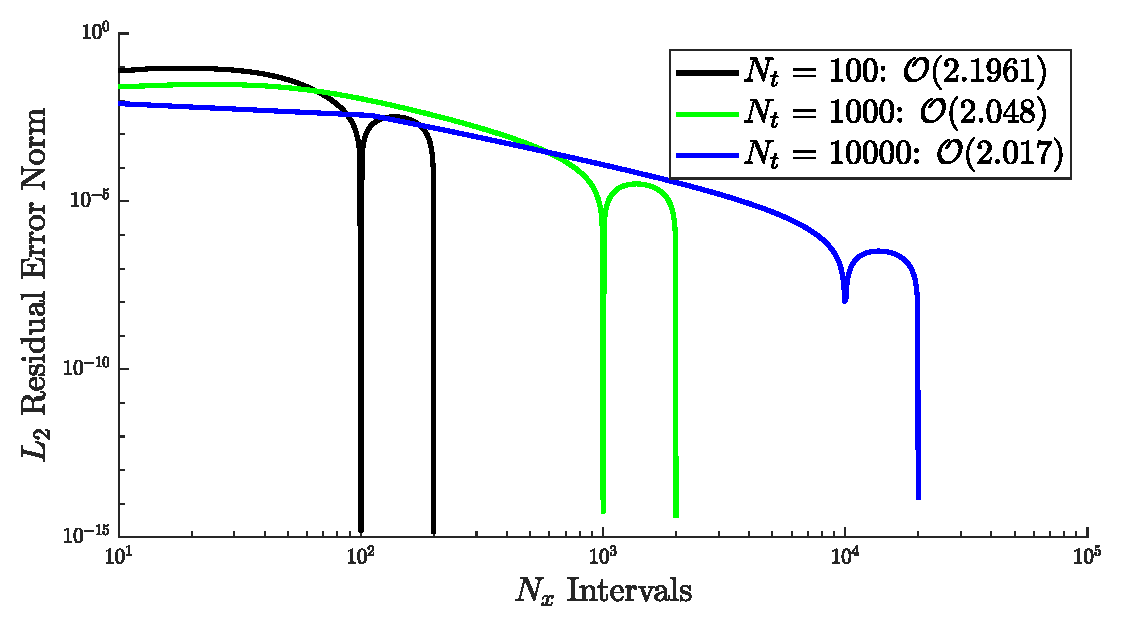
\includegraphics[width = 0.9\linewidth]{q2/BW_convergence.eps}
        \caption{Beam-Warming implementation and convergence of spatial and temporal convergences.}
        \label{fig:q2_BW}
    \end{figure}


    \begin{fminipage}{0.9\linewidth}
        \textbf{Shown above in Figure \ref{fig:q2_BW} are the convergences of the $\bf L_2$ norm. As $\bf N_x$ increases for each given $\bf N_t$ value, it will reach the CFL number stability limits of $\bf \sigma = 1,\ 2$. When $\bf \sigma = 1$ for each combination of $\bf N_x,\ N_t$ it is seen as the vertical asymptote in which the residual norm decreases significantly. Computing the orders of accuracy in the spatial domain confirms that this scheme is second-order accurate in the spatial domain such that $\bf \mathcal{O}(\Delta x^2)$. Looking at the temporal convergence can be done through visual inspection to be first order accurate $\bf \mathcal{O}(\Delta t)$, but will be shown on the following page.}
    \end{fminipage}

    \vfill
    Continued on the next page\ldots

    \pagebreak

    Implementing the Beam-Warming method again but only varying $N_t$ gives that the spatial convergence below in Figure \ref{fig:q2_BW_nt},

    \begin{figure}[h]
        \centering
        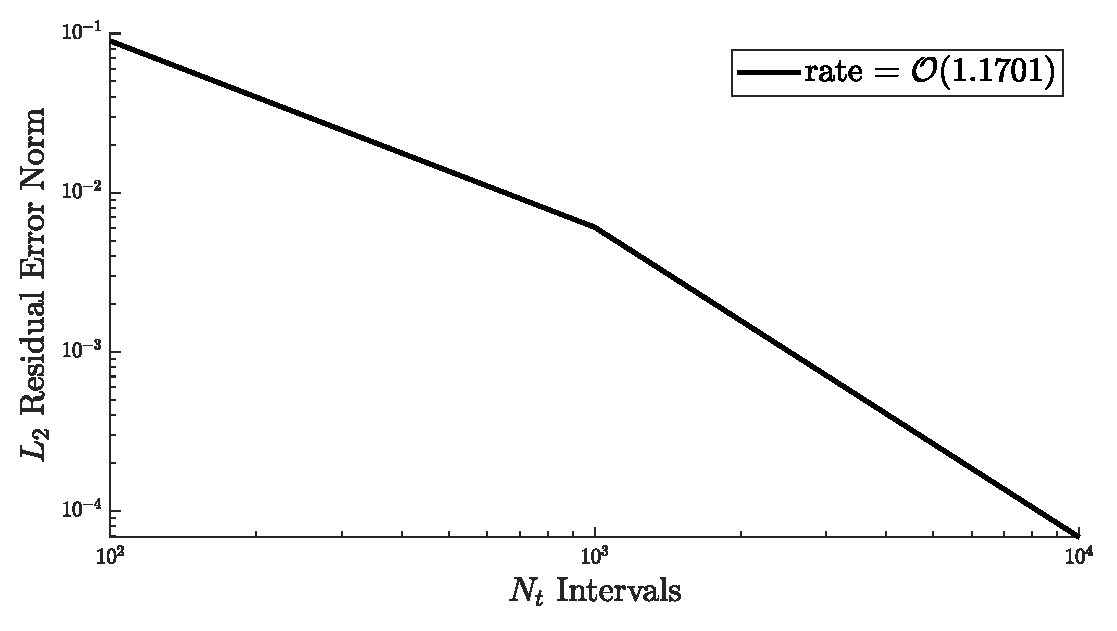
\includegraphics[width = 0.9\linewidth]{q2/BW_convergence_nt.eps}
        \caption{Temporal only convergences of Beam-Warming method.}
        \label{fig:q2_BW_nt}
    \end{figure}

    \begin{fminipage}{0.9\linewidth}
        \textbf{Shown above in Figure \ref{fig:q2_BW_nt} are the temporal convergences of the Beam-Warming method. Again it is shown and confirmed that it is first-order accurate.}
    \end{fminipage}



\end{enumerate}